\subsubsection{Data Augmentation}
    Generally, when using Machine Learning for classification problems, it is more ideal to learn a classifier that can perform well on a population. 
    An example of a population would be the set of all handwritten characters in the entire world. Generally, that complete population will not always be available for training, we only have a much smaller training dataset. 
    If a training set is large enough, it might be a good approximation of the population we're interested in, but it's still just that, an approximation.
    
    A learning algorithm is over-fitting if it performs significantly better on the training set than it is on the population (which will be generally approximated again using a separate test set).
    
    To help combat over-fitting and data deficiency, along with increasing the model's accuracy, Data Augmentation techniques are used to diversify existing data points.
    Data augmentation is an effective method for enhancing the performance of our computer vision models without having to collect more data.
    \label{Figure Data Augmentation}
\begin{figure}[H]
    \centering
    \begin{subfigure}{0.15\textwidth}
        \centering
        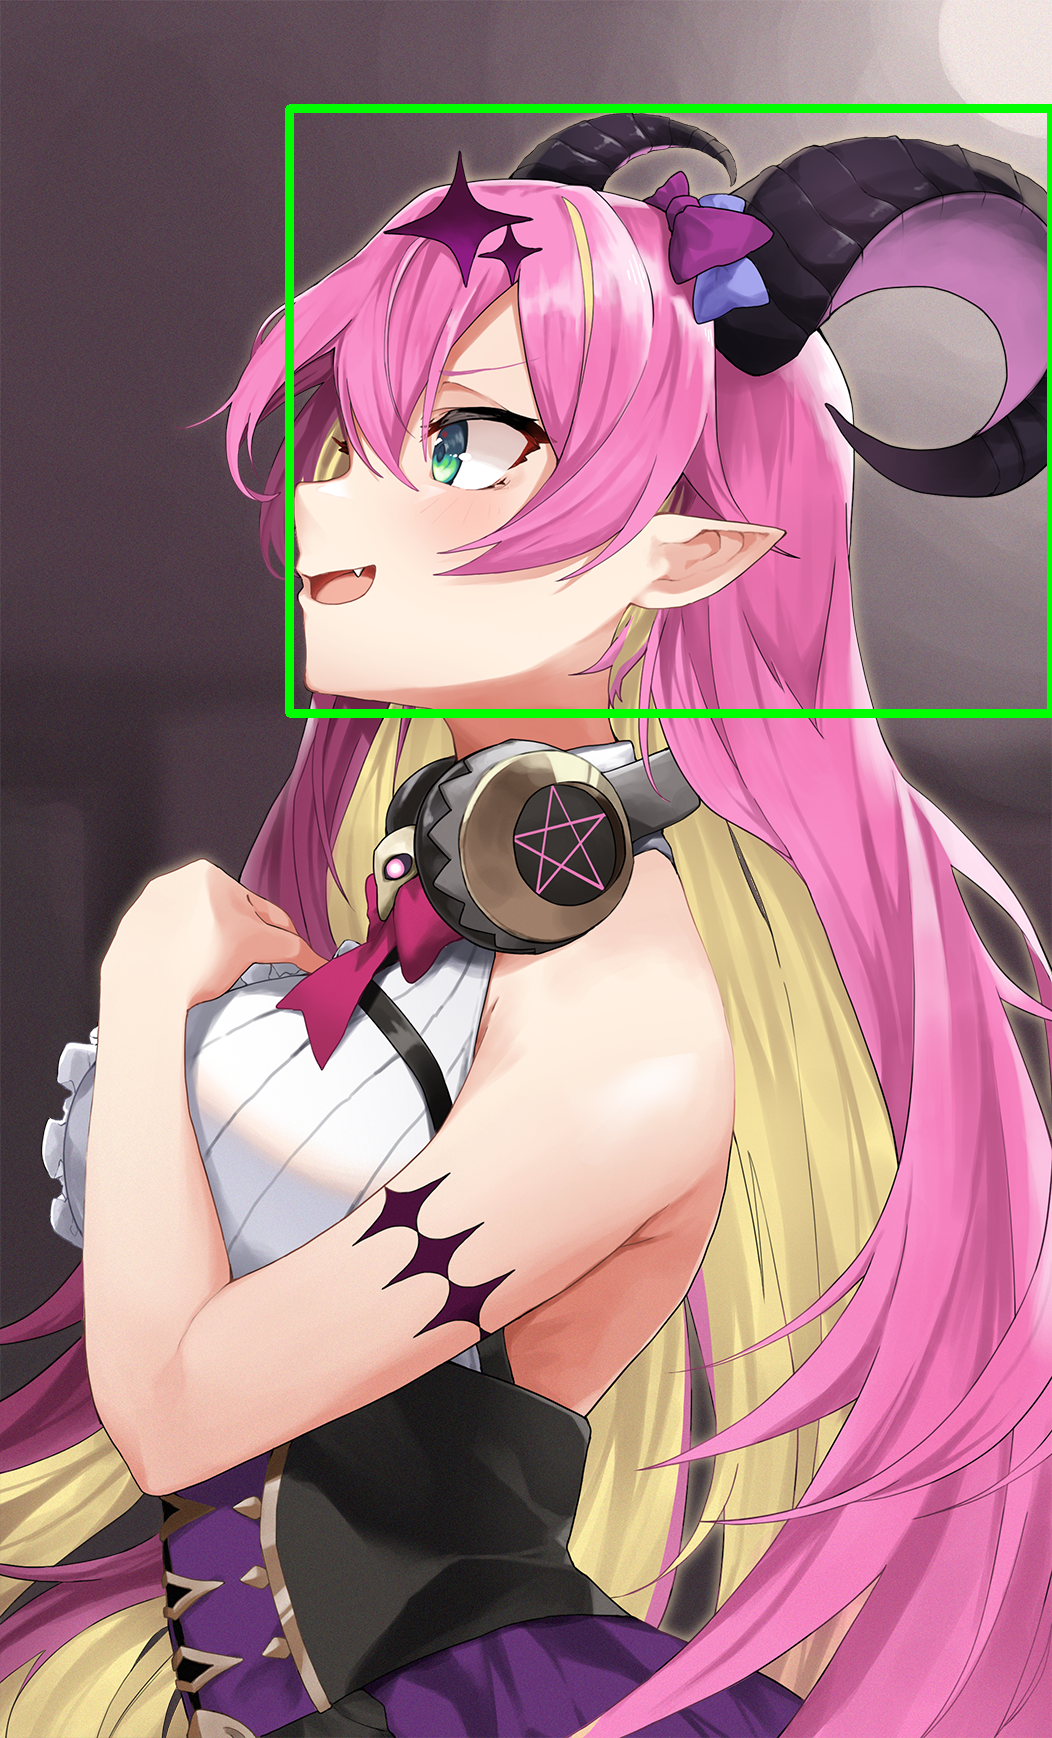
\includegraphics[width=\textwidth]{images/augmentation/Pixiv-83768702_p0-BB.png}
        \caption{}
        \label{fig:aloe1}
    \end{subfigure}
    \hfill
    \begin{subfigure}{0.15\textwidth}
        \centering
        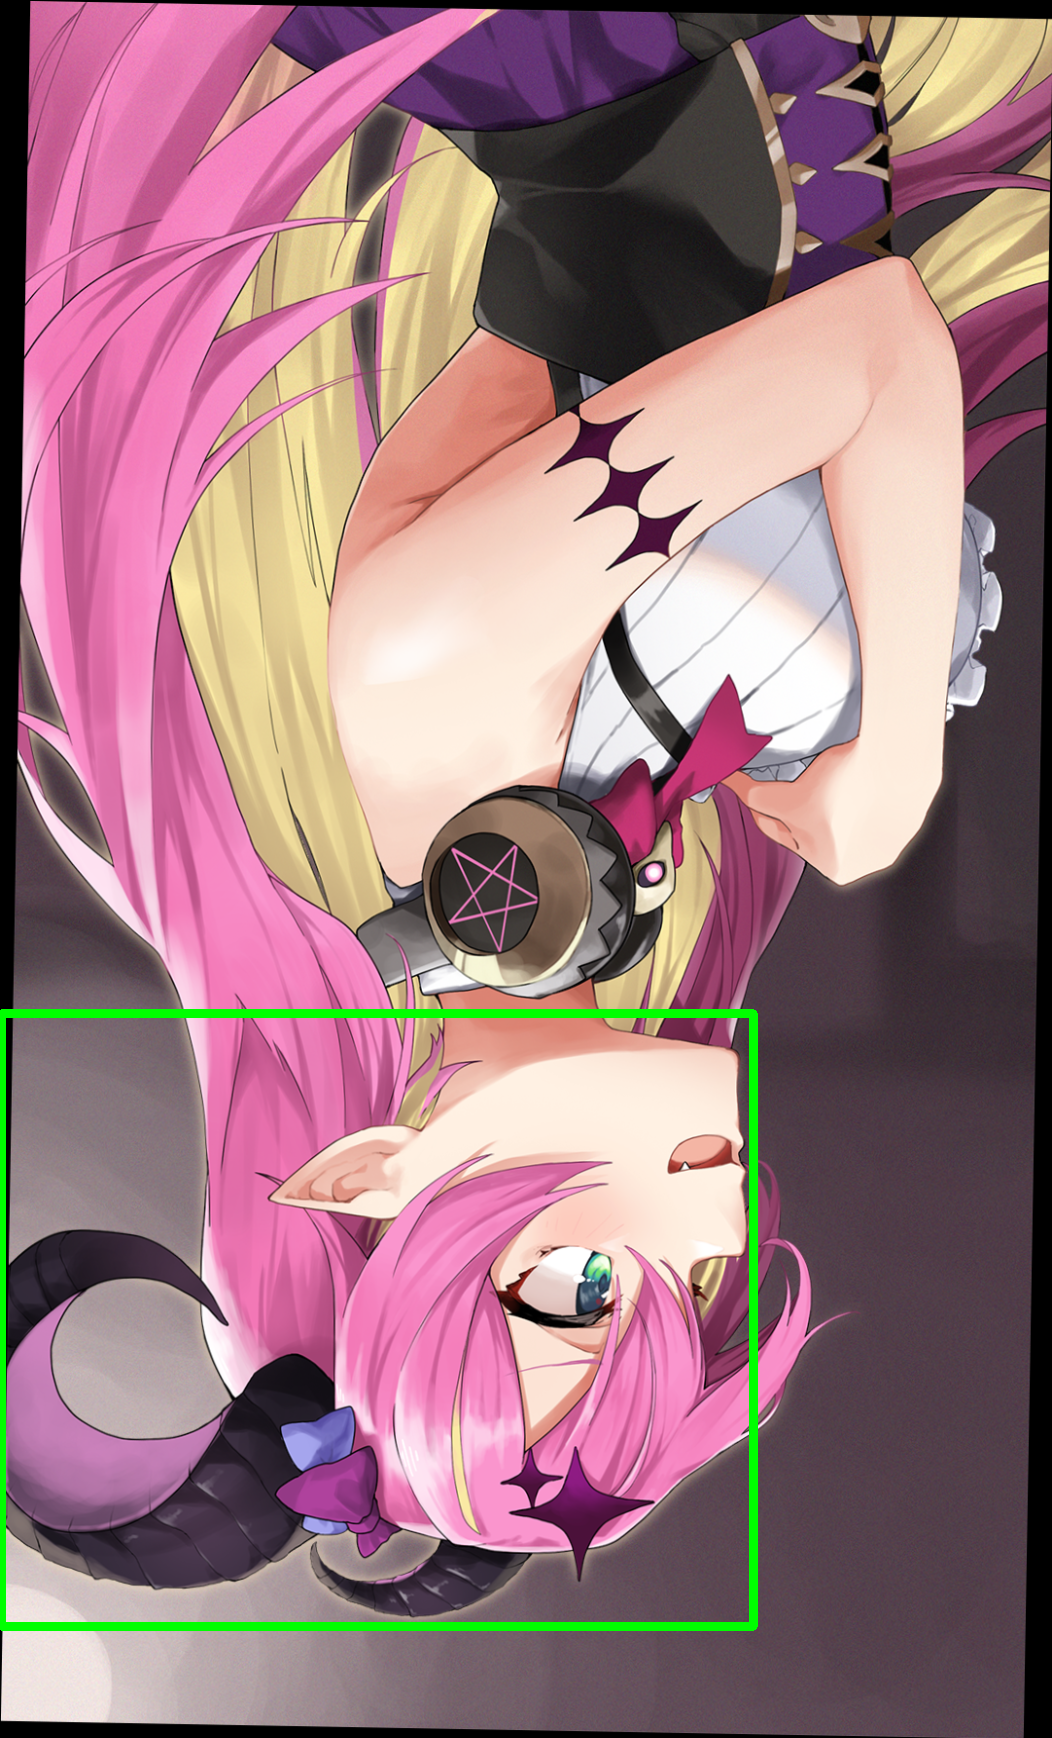
\includegraphics[width=\textwidth]{images/augmentation/Pixiv-83768702_p0-RandomRotate_179-BB.png}
        \caption{}
        \label{fig:aloe2}
    \end{subfigure}
    \hfill
    \begin{subfigure}{0.15\textwidth}
        \centering
        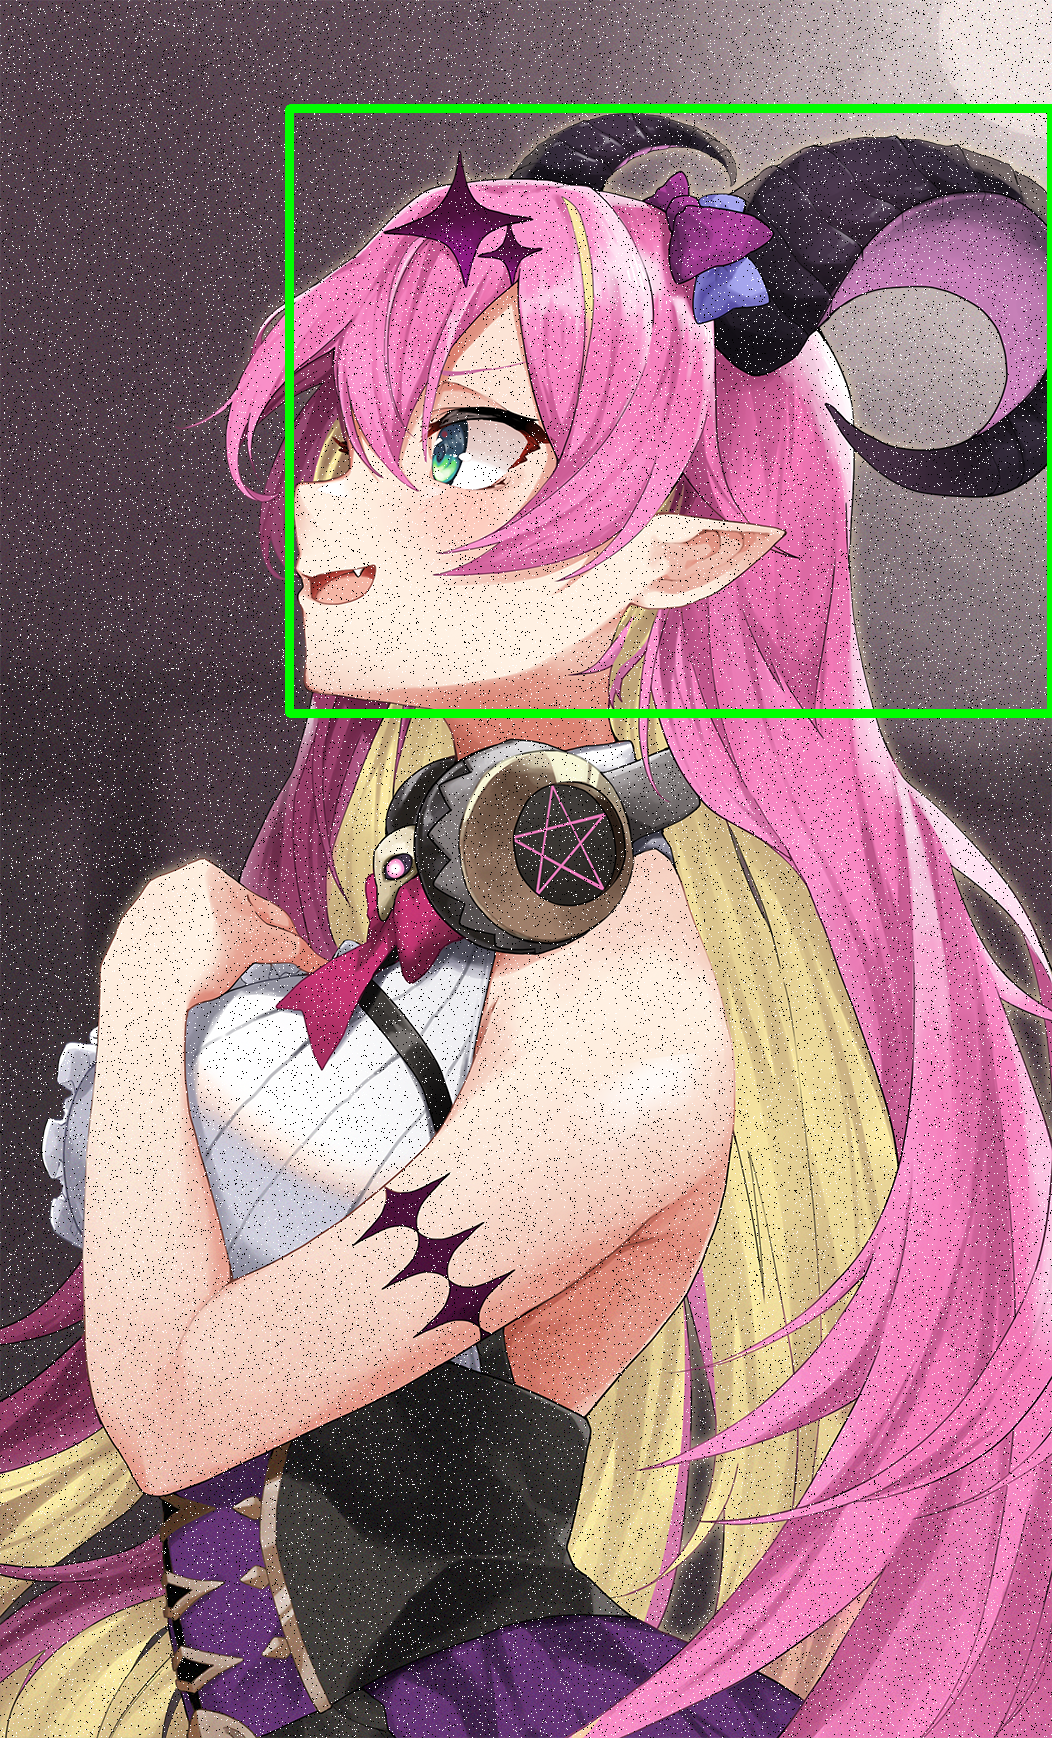
\includegraphics[width=\textwidth]{images/augmentation/Pixiv-83768702_p0-RandomSaltAndPepper_0.044-BB.png}
        \caption{}
        \label{fig:aloe3}
    \end{subfigure}
    \hfill
    \begin{subfigure}{0.15\textwidth}
        \centering
        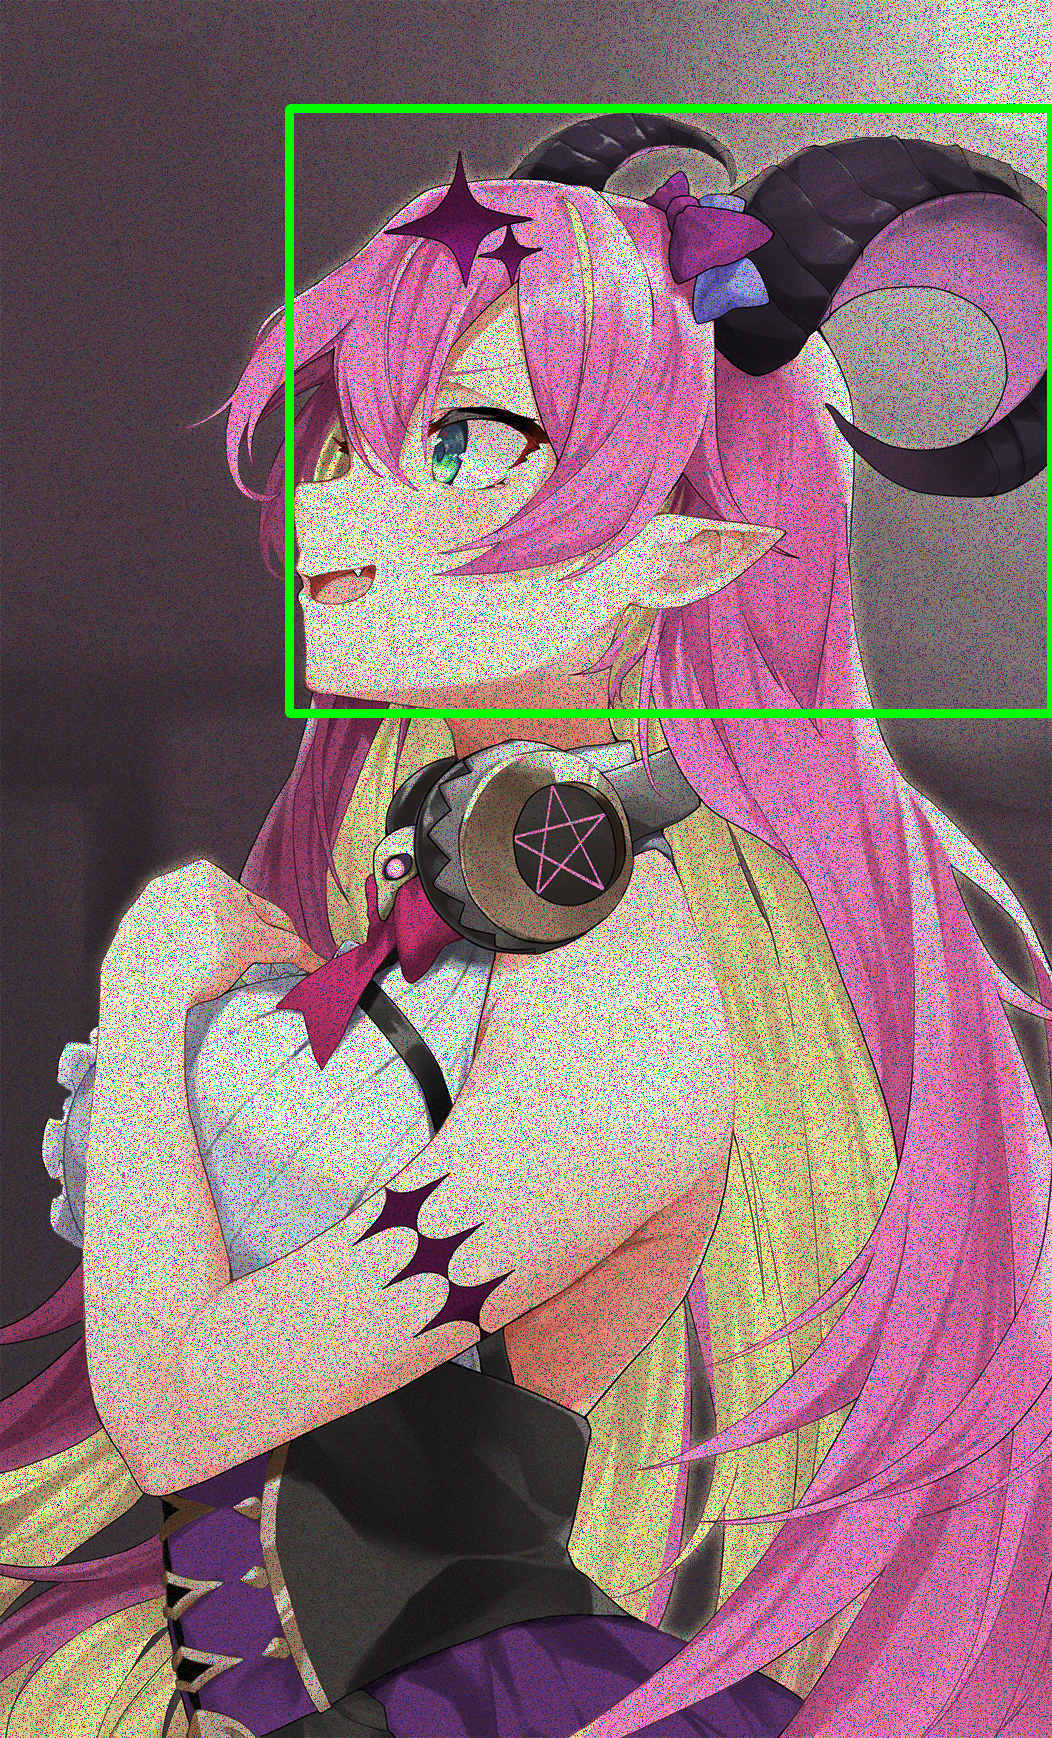
\includegraphics[width=\textwidth]{images/augmentation/Pixiv-83768702_p0-RandomValuedImpulseNoise_0.138-BB.png}
        \caption{}
        \label{fig:aloe4}
    \end{subfigure}
    \begin{subfigure}{0.15\textwidth}
        \centering
        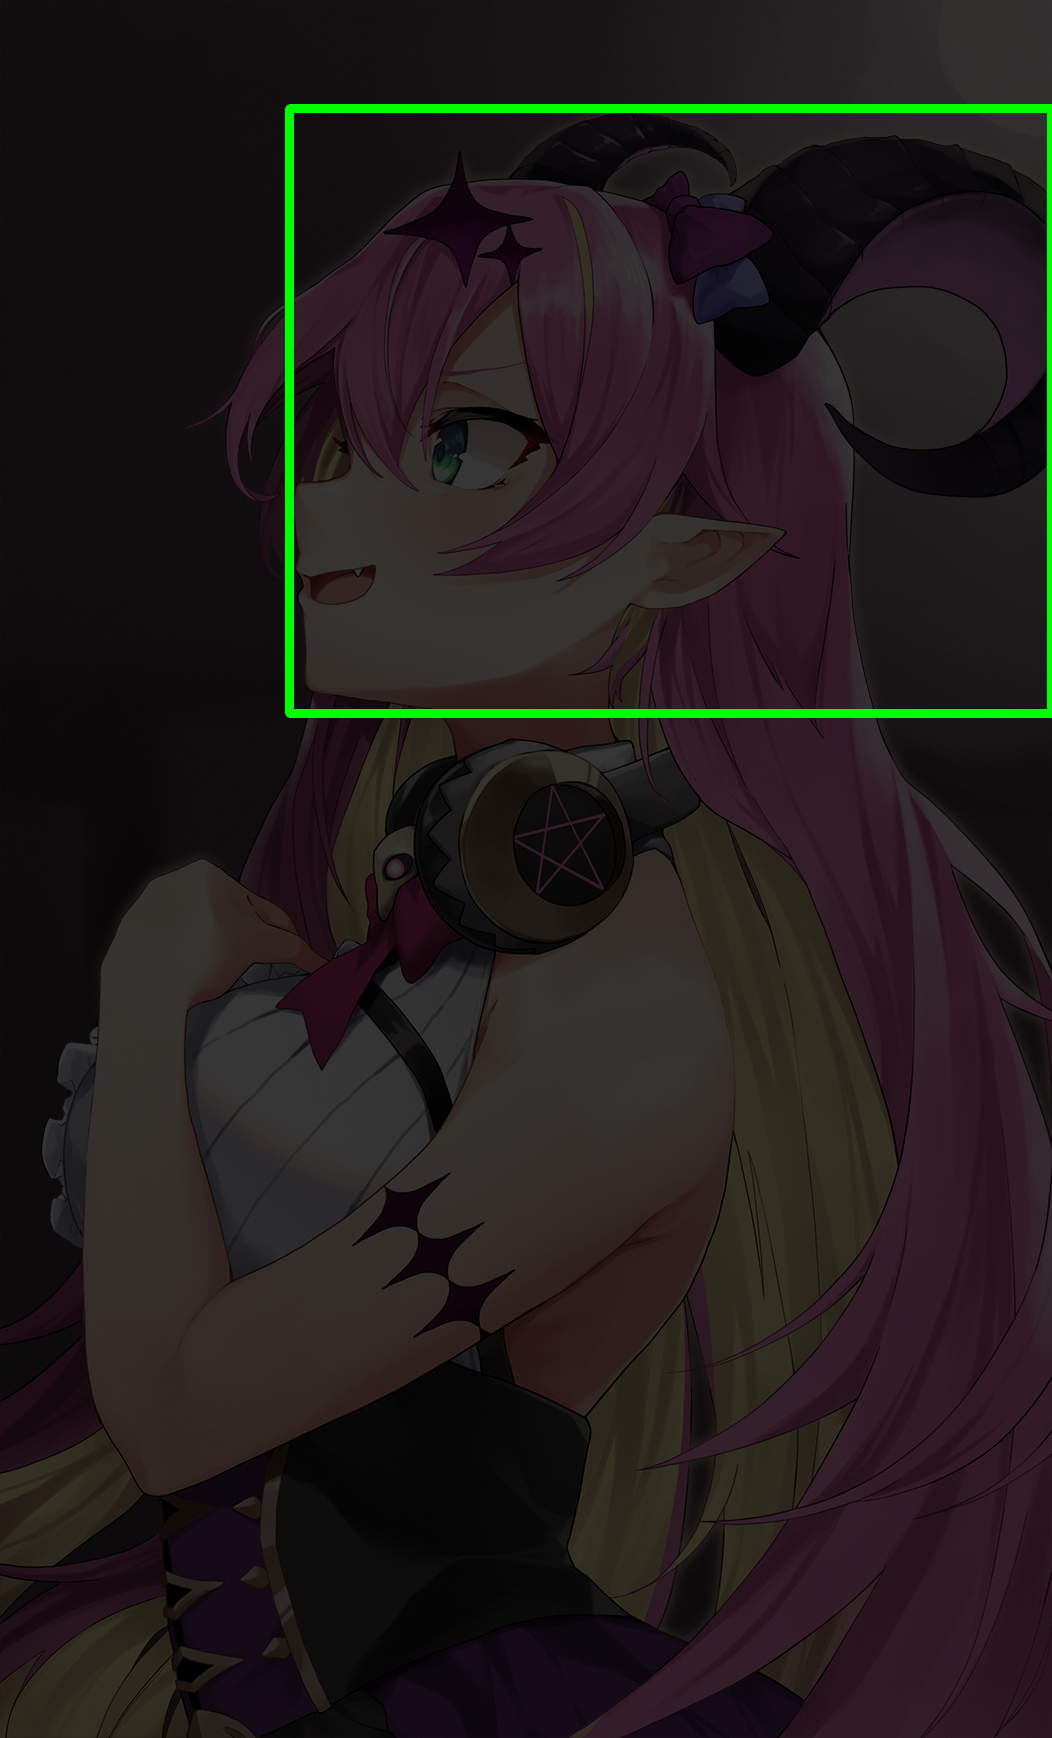
\includegraphics[width=\textwidth]{images/augmentation/Pixiv-83768702_p0-RandomBrightness_0.213-BB.png}
        \caption{}
        \label{fig:aloe5}
    \end{subfigure}
    \begin{flushleft}
        (a) Original image\cite{83768702}\\
        (b) Rotate 179 degrees\\
        (c) Random Salt and Pepper with 4.4\% \\
        (d) Random Valued Impulse Noise with 13.8\% \\
        (e) Brightness with intensity 0.213\\
    \end{flushleft}
    \caption{Data augmentation methods}
    \label{fig:manoaloe1}
\end{figure}
    \paragraph{Random-valued Impulse Noise, Salt and Pepper}
        Real-world data is seldom clean. At least it is not as clean as the data that we train our model on. 
        Noise in the data can reduce the accuracy of the model and lead to less generalization power. 
        This is the main reason why many times deep neural network models perform poorly during testing. 
        Therefore, noise are used to augment data. Not only will there be more data to use for training, 
        but the noisy data used for training the model will also make it better at generalizing real-world noisy data.
        \begin{lstlisting}[language=Python]
mask = np.random.rand(*self.image.shape[:2])
mask = np.concatenate([mask, mask, mask])
mask = mask.reshape(*mask.shape, 3)
self.image = np.where(
                self.portion*2>mask,
                np.random.randint(low=0, 
                                  high=255, 
                                  size=1, 
                                  dtype=int),
                self.image) 
        \end{lstlisting}
% =========================================================
    \paragraph{Random Brightness}
         Training the model with images with various luminosity will help it better generalize images that are not trained even on different lighting conditions\cite{RandomBrightness}. 
         The brightness and darkness depend upon one boundary value which is 1.0.
         At 1.0, the image will be in its original state.
         If the value is less than 1.0 then it will darken the image like [0.1,1.0), whereas a value greater than 1.0 makes the image brighter like (1.0, 2.0].
         At level 0 of luminosity, the image is filled with black pixels.
         \begin{lstlisting}[language=Python]
img = (self.image * self.level).astype(int)
self.image = np.clip(a=img,
                     a_min=0,
                     a_max=255)
         \end{lstlisting}
% =========================================================
    \paragraph{Image rotation}
        \label{Figure Rotation Formula}
\begin{figure}[H]
    \centering
    \includegraphics[width=0.4\textwidth]{Picture2.png}
    \label{fig:pic2}
    \begin{center}
        \begin{align*}
            N_{w} = h * \sin(\theta) + w * \cos(\theta)\\
            N_{h} = h * \cos(\theta) + w * \sin(\theta)
        \end{align*}
    \end{center}
    \caption{Rotation Formula}
\end{figure}
        \label{Figure Image Rotation}
\begin{figure}[H]
    \centering
    \begin{subfigure}{0.15\textwidth}
        \centering
        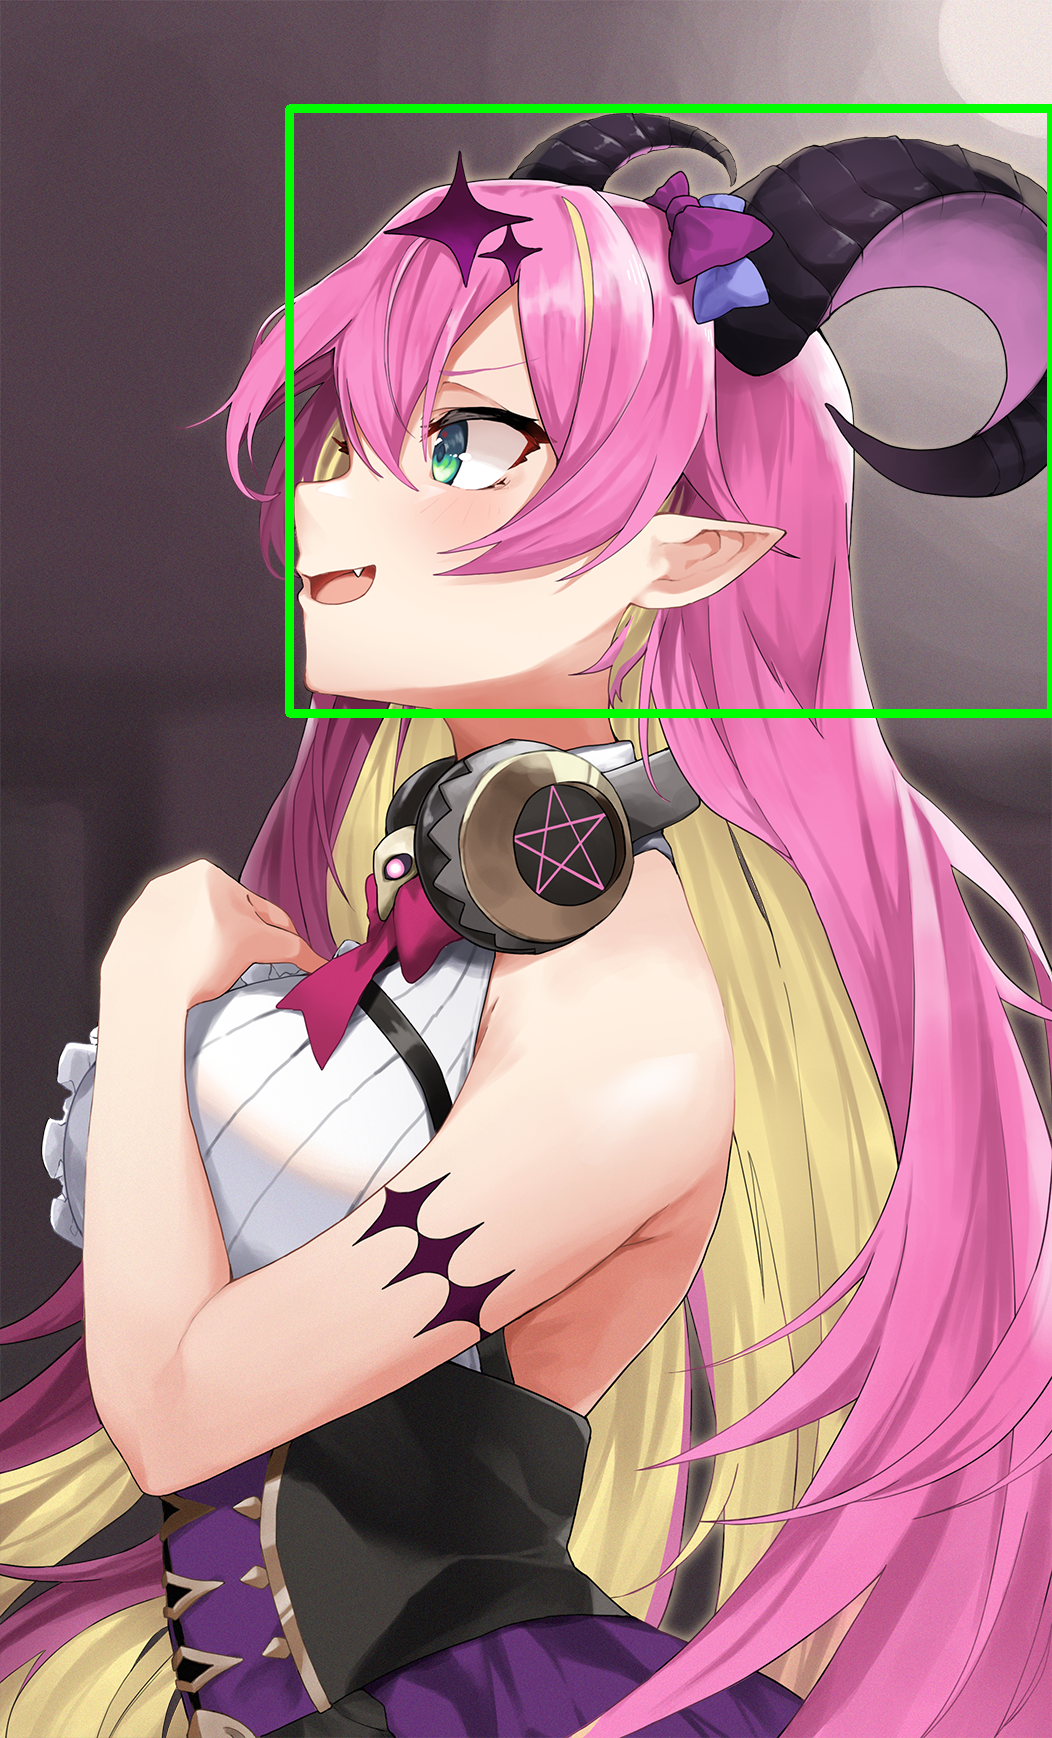
\includegraphics[width=\textwidth]{images/augmentation/Pixiv-83768702_p0-BB.png}
        % \caption{Original}
        \caption{}
        \label{fig:aloe1}
    \end{subfigure}
    \hfill
    \begin{subfigure}{0.15\textwidth}
        \centering
        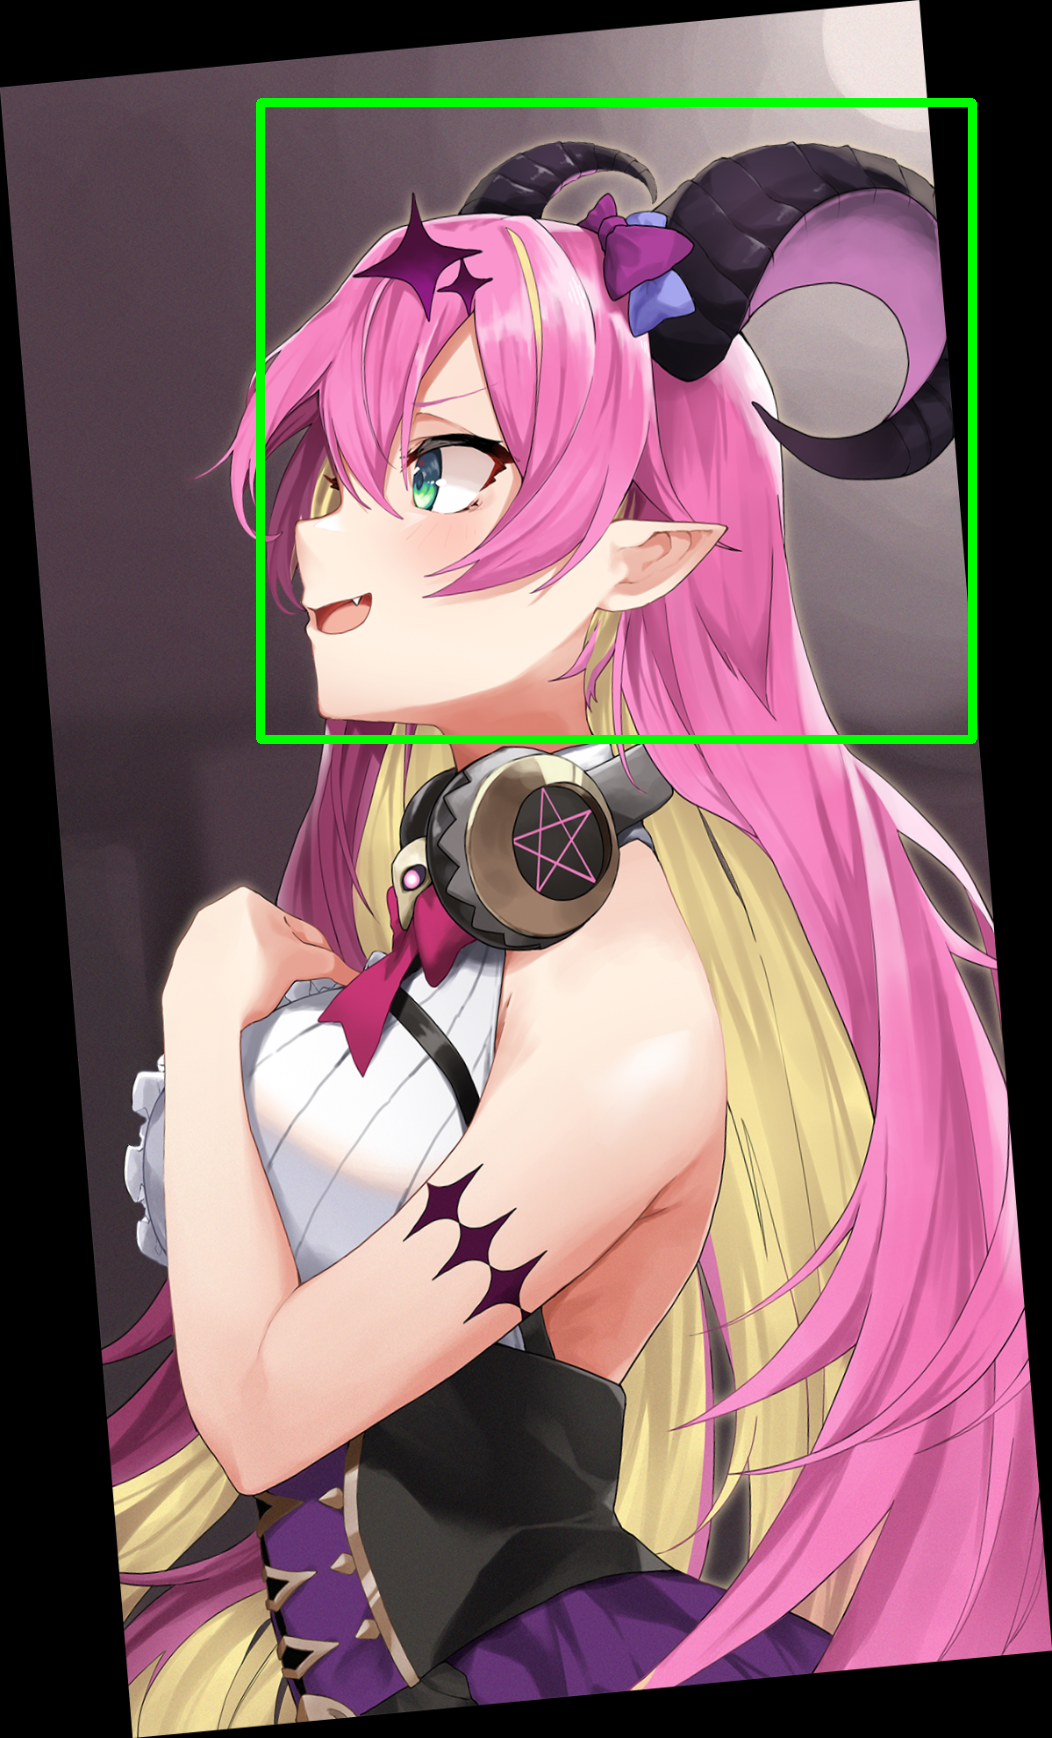
\includegraphics[width=\textwidth]{images/augmentation/Pixiv-83768702_p0-RandomRotate_5-BB.png}
        % \caption{5 degrees}
        \caption{}
        \label{fig:aloe2}
    \end{subfigure}
    \hfill
    \begin{subfigure}{0.15\textwidth}
        \centering
        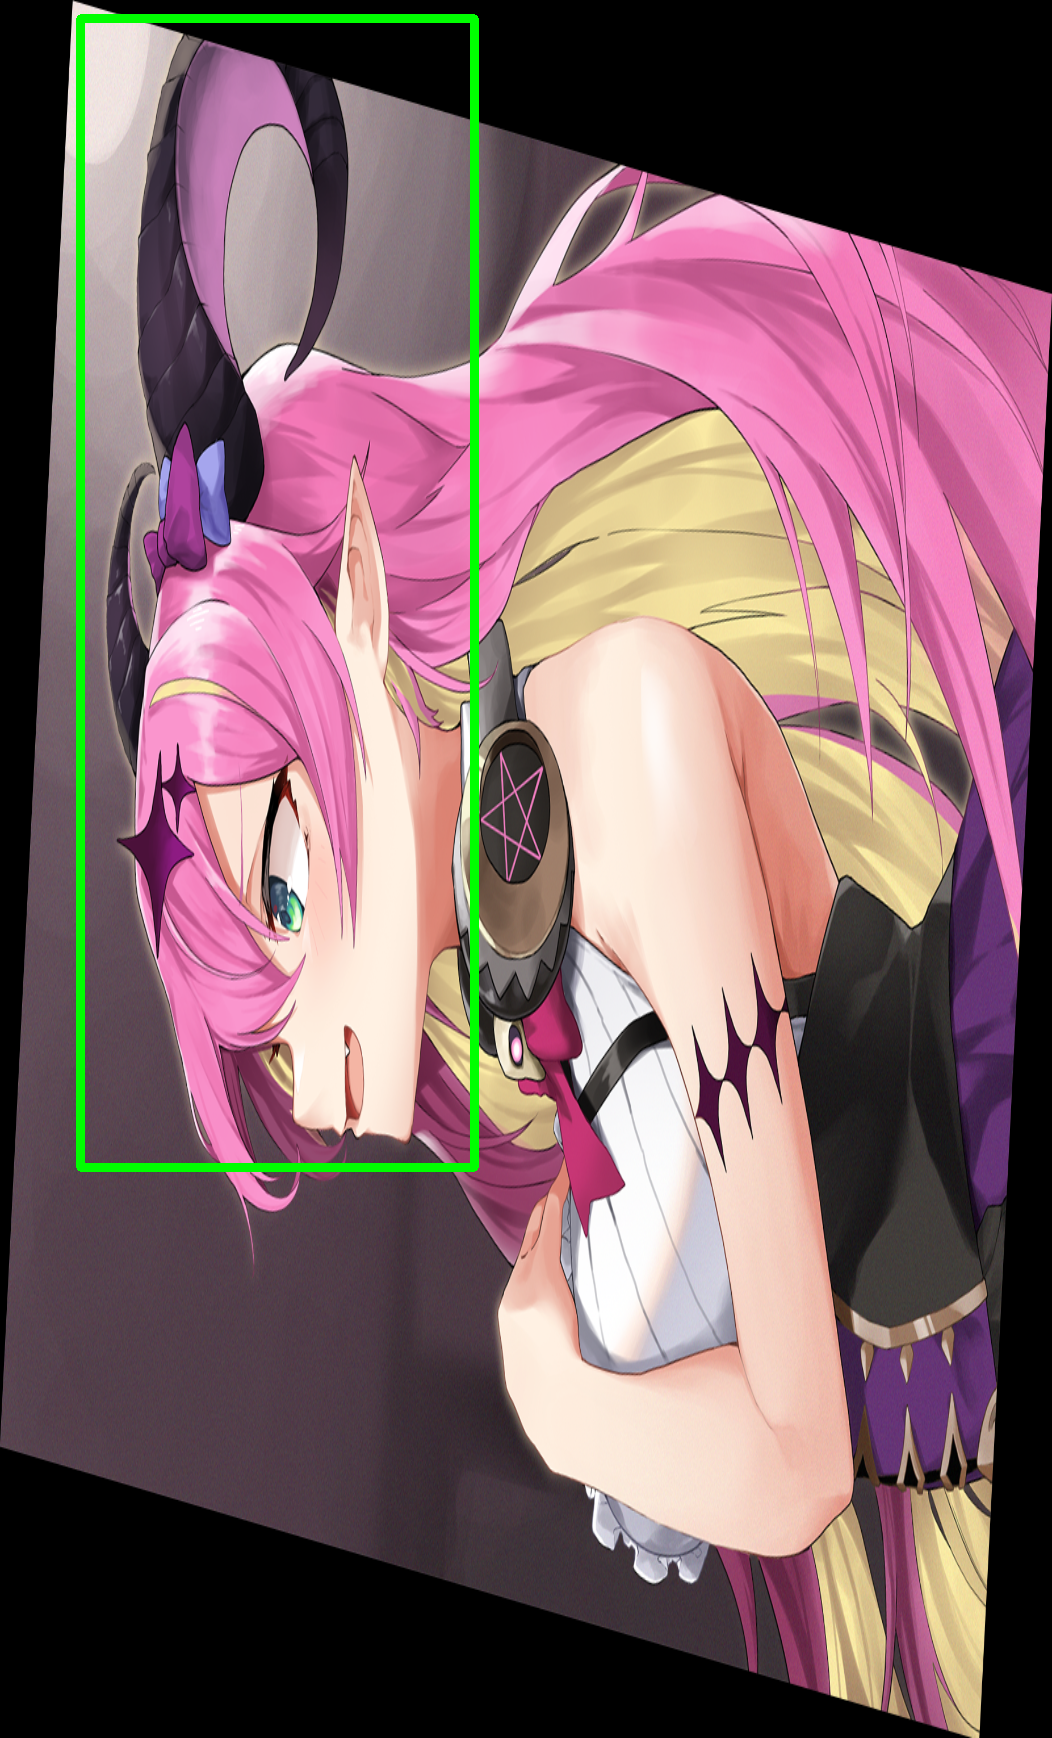
\includegraphics[width=\textwidth]{images/augmentation/Pixiv-83768702_p0-RandomRotate_83-BB.png}
        % \caption{83 degrees}
        \caption{}
        \label{fig:aloe3}
    \end{subfigure}
    \hfill
    \begin{subfigure}{0.15\textwidth}
        \centering
        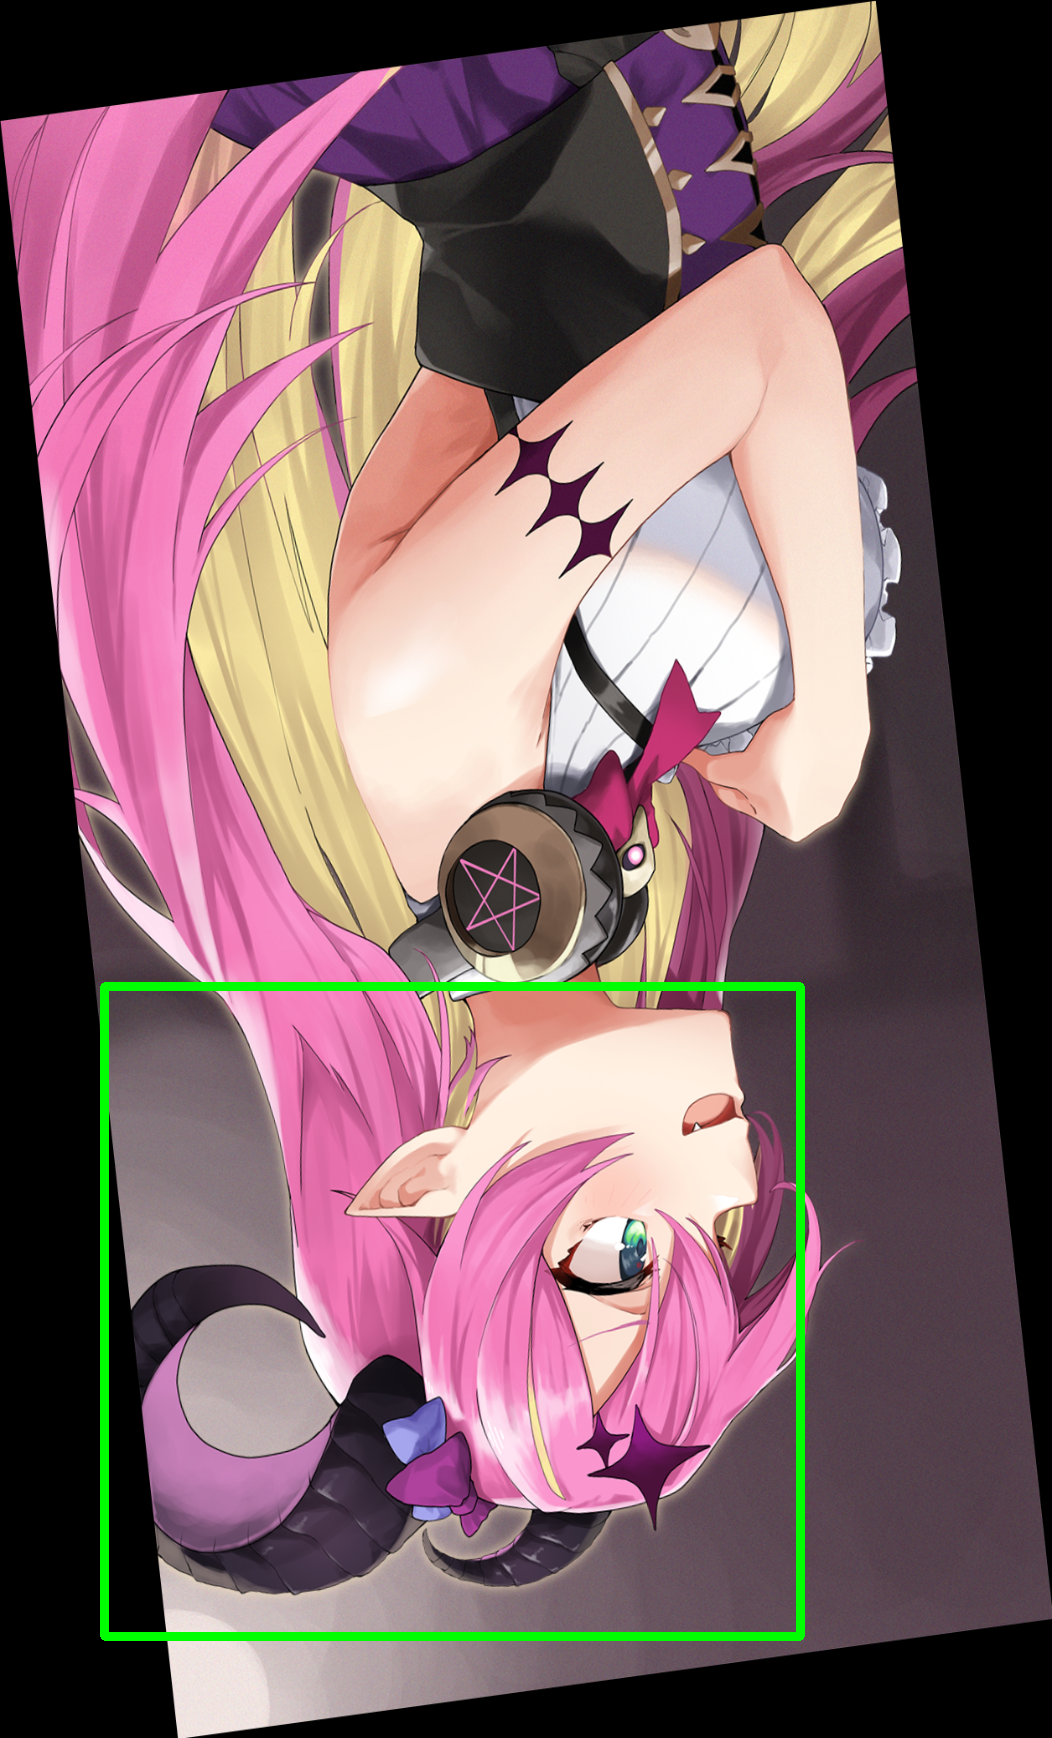
\includegraphics[width=\textwidth]{images/augmentation/Pixiv-83768702_p0-RandomRotate_187-BB.png}
        % \caption{187 degrees}
        \caption{}
        \label{fig:aloe4}
    \end{subfigure}
    \begin{subfigure}{0.15\textwidth}
        \centering
        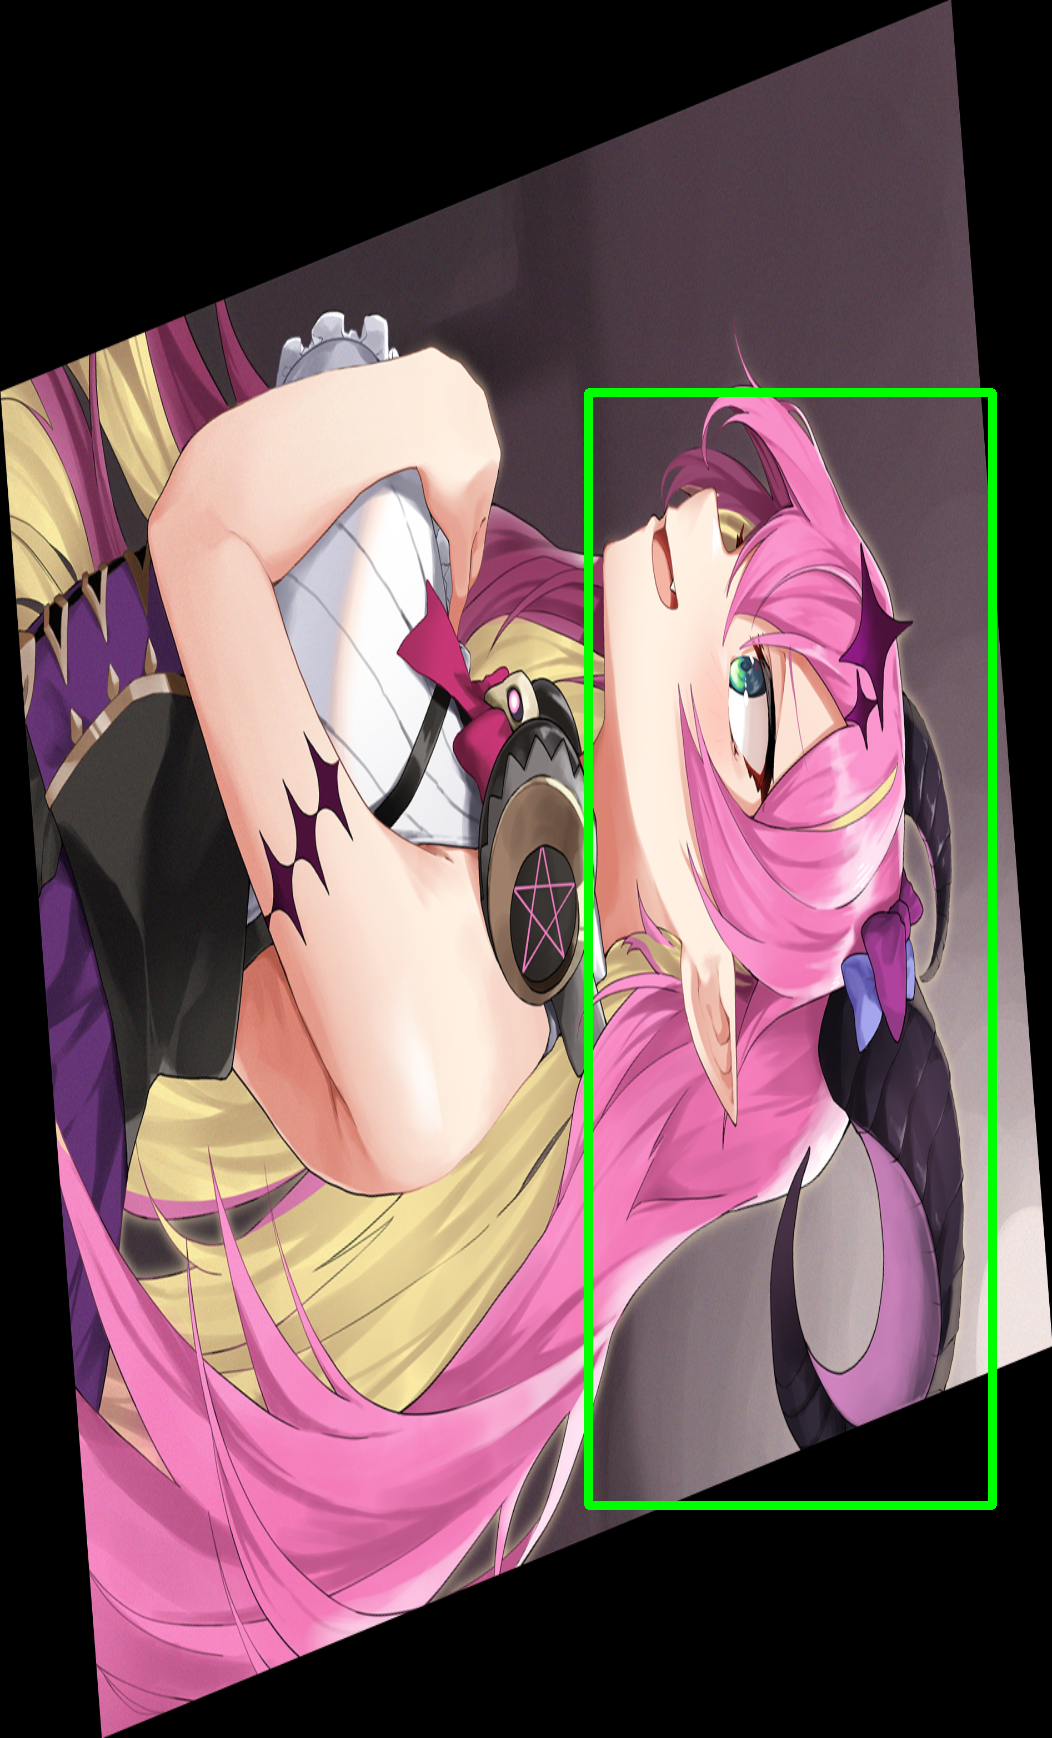
\includegraphics[width=\textwidth]{images/augmentation/Pixiv-83768702_p0-RandomRotate_280-BB.png}
        % \caption{280 degrees}
        \caption{}
        \label{fig:aloe5}
    \end{subfigure}
    \begin{flushleft}
        (a) Original image\cite{83768702}\\
        (b) Rotate with 5 degrees\\
        (c) Rotate with 83 degrees\\
        (d) Rotate with 187 degrees\\
        (e) Rotate with 280 degrees\\
    \end{flushleft}
    \caption{Image Rotation}
    \label{fig:manoaloe1}
\end{figure}
        Because it alters the angles at which objects appear in the dataset during training, Random Rotate is a particularly helpful augmentation. 
        Perhaps images were only taken with an item horizontally throughout the image gathering phase, but the object could have been skewed in any direction during manufacturing. 
        However, this method is by far the most sophisticated. 
        The items in an image are also relocated when it is rotated.
        However fortunately, we discovered a tutorial by Ayoosh Kathuria that can assist us in solving this issue with just some modification\cite{Rotation}.